\documentclass[12pt, letterpaper]{article}
\usepackage[utf8]{inputenc}
\usepackage[left = 2.5cm, right = 2.5cm, top = 2.5cm, bottom = 2.5cm]{geometry}
\usepackage{amsthm}
\usepackage{amsfonts}
\usepackage{amsmath}
\usepackage{amssymb}
\usepackage{graphicx}
\usepackage{color}
\usepackage[T1]{fontenc}
\graphicspath{{consultas/}}

\author{Hernández Ferreiro Enrique Ehecatl (315020904) \\
        López Soto Ramses Antonio (315319974) \\
        Miguel Torres Eric Giovanni (315230190) \\
        Quintero Villeda Erik (315199345)}

\title{Tarea 6: Lenguaje de consultas SQL \\
       {\small Fudamentos de Bases de Datos}}

\date{17 de noviembre de 2019}


\definecolor{dkgreen}{rgb}{0,0.6,0}
\definecolor{ltgray}{rgb}{0.5,0.5,0.5}


\begin{document}
\maketitle

Se tiene el siguiente esquema de base de datos acerca de empleados, los lugares donde trabajan y los proyectos que desarrollan:

\begin{center}
	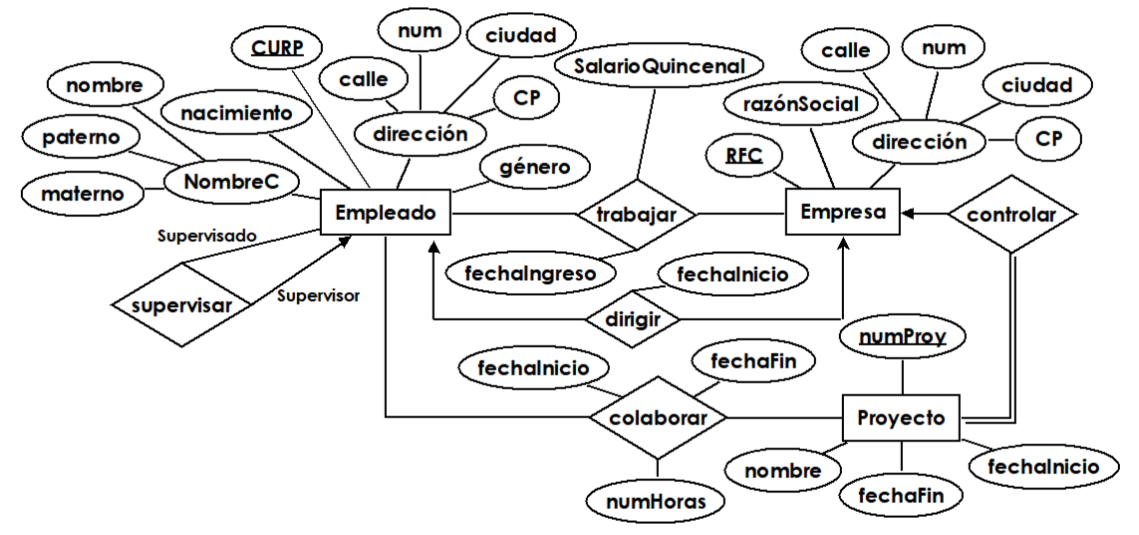
\includegraphics[scale=0.2]{meTrabajo.png}
\end{center}

Resuelve los siguientes puntos:

\begin{itemize}
	\item[1.] Traduce el modelo \textbf{E-R} a su correspondiente \textbf{modelo relacional} indicando claramente las 
			  \textbf{llaves primarias y foráneas}. No incluyas relaciones redundantes.
			
				\begin{center}
					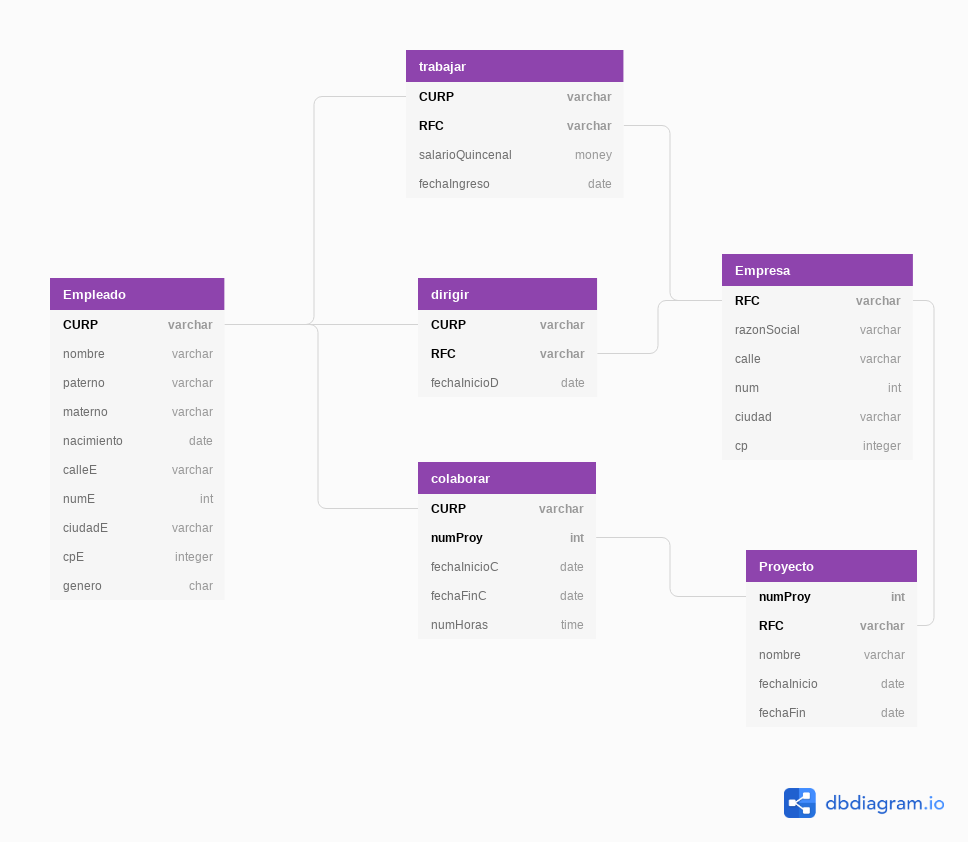
\includegraphics[scale=0.2]{Trabajo.png}
				\end{center}
	
	\item[2.] Proporciona un \textbf{script en SQL} que contenga el \textbf{esquema de cada tabla} incluyendo las \textbf{restricciones
			  de integridad} que consideres necesarias. Deberás incluir la \textbf{totalidad de restricciones} que se hayan
	          revisado en clase y/o en laboratorio y debe ser un esquema con \textbf{Integridad Referencial}; deberás
			  agregar alguna \textbf{política de mantenimiento de FK}.
			  
		

		\item[3.] Proporcionar un script en SQL que permita poblar el esquema anterior. \\
		Deberás tener información, para al menos 100 compañías (una de ellas debe ser PEMEX), 500
		empleados y no menos de 50 proyectos. El 20\% de los empleados deberán estar distribuidos en al
		menos 10 ciudades diferentes y algunos de ellos deben vivir en la misma ciudad que trabajan.

		\item[4.] Proporcionar un script en SQL con la solución a cada una de las siguientes consultas
		
			\begin{itemize}
			    \item[a.] Encontrar el nombre y la ciudad de todos los empleados que trabajan en PEMEX
			
				\item[b.] Encontrar todos los empleados que no viven en la misma ciudad de la empresa en que
				trabajan.

				\item[c.] Calcular el salario mensual de todas las directoras.

				\item[d.] Obtener la información de los directores (en general) y empresas que comenzaron a dirigir
				durante el segundo y cuarto trimestre de 2018.

				
				\item[e.] Encontrar a todos los empleados que viven en la misma ciudad y en la misma calle que su
				supervisor.

			
				\item[f.] Obtener una lista de cada compañía y el salario promedio que paga. La información se debe
				mostrar por compañía, año, y género.


				\item[g.] Empleados que colaboran en proyectos que controlan empresas para las que no trabajan.


				\item[h.] Encontrar el máximo, mínimo y total de salarios pagados por cada compañía.


				\item[i.] Encontrar información de los empleados y número de horas que dedican a los proyectos.
				Interesan aquellos empleados que colaboran en al menos dos proyectos y en donde el
				número de horas que dediquen a algún proyecto sea mayor a 20.

				\item[j.] Encontrar la cantidad de empleados en cada compañía, por año, trimestre y género.


				\item[k.] Encontrar el nombre del empleado que gana más dinero en cada compañía.

				\item[l.] Obtener una lista de los empleados que ganan más del salario promedio que pagan las
				compañías.

					
				\item[m.] Encontrar la compañía que tiene menos empleados y listar toda la información de los mismos.

				\item[n.] Información de los proyectos en los que colaboran los empleados que son directores.

				\item[o.] Encontrar la compañía que tiene empleados en cada una de las ciudades que hayas
				definido.

				\item[p.] Empleados que dejaron de colaborar en proyectos, antes de la fecha de finalización de los
				mismos.


				\item[q.] Información de los empleados que no colaboran en ningún proyecto.

				\item[r.] Encontrar la información de las compañías que tienen al menos dos empleados en la misma
				ciudad en que tienen sus instalaciones.

				\item[s.] Proyecto que más empleados requiere (o requirió) y el número de horas que éstos le
				dedicaron.

				\item[t.] Empleados que comenzaron a colaborar en proyectos en la misma fecha de su cumpleaños.


				\item[u.] Obtener una lista del número de empleados que supervisa cada supervisor.

				\item[v.] Obtener una lista de los directores de más de 50 años.

				\item[w.] Obtener una lista de los empleados cuyo apellido paterno comience con las letras A, D, G, J,
				L, P o R.


				\item[x.] Número de empleados que colaboran en los proyectos que controla cada empresa para
				aquellos proyectos que hayan iniciado en diciembre.
				\item[y.] Crea una vista con la información de los empleados y compañías en que trabajan, de aquellos
				      empleados que lo hagan en al menos tres compañías diferentes.	
			\end{itemize}
			                

			
		\item[5.] Indica para la política de mantenimiento de llaves foráneas, qué ventajas y desventajas que tienen
		las políticas de establecimiento de nulos y cascada. \vspace{.2cm}

		CASCADE \\
		Si esa fila se actualiza o elimina en la tabla primaria, las filas correspondientes se actualizan o eliminan en la tabla de referencia.\vspace{.3cm}

		SET NULL \\
        Cuando se actualiza o elimina la fila correspondiente en la tabla primaria, todos los valores que componen la clave externa se establecen en NULL. Para que esta restricción se ejecute, las columnas de clave externa deben aceptar valores NULL.
\end{itemize}


\end{document}

